\documentclass[12pt,a4paper]{IEEEtran}
\usepackage[latin1]{inputenc}
%% Useful packages
\usepackage{amsmath}
\usepackage{graphicx}
%%
\title{Control I \\ {\sc Modelado de sistemas de primer orden} }
\author{ Profesor  \\ Gerardo Marx Cháve-Campos\\ Alumnos \\ Aracely lizeth Hernandez Arteaga 14121092 \\ Erick David Bedolla García 14121081\\ Instituto Tecnologíco de Morelia \\ Departamento de Electrónica}
\begin{document}
\maketitle
\tableofcontents
\section{Resumen}
En esta práctica analizamos los modelos de sistemas de primer orden de un sistema hidráulico, también implementamos un programa en scilab para ver la respuesta de este a una función escalon.
\section{Introducción}
El control a desempeñado un papel muy importante en el avance de la tecnología y procesos indutriales. Algunas de las ramas que han tenido un avance significativo son los sistemas de vehiculos espaciales, en los sistemas roboticos, en procesos modernos de fabricación cualquier operación industrial que requiera el control de temperatura, presión, humedad, flujo,etc.\cite{Ogata} \\
Estos sistemas pueden ser representados por un modelo matemático el cual es un conjunto de ecuaciones que pueden representar el comportamiento del sistema. Estos sistemas pueden ser dinámicos, eléctricos, mecánicos, entre otros más. \\
Estos modelos pueden variar según la persepectiva se tenga del problema planteado.\cite{Ogata}
\\ \\
Los sistemas se pueden dividir depende el modelado matemático que este tenga puede ser de orden uno , dos, ... n. Donde entre más alto es el orden más complicado es resolverlo ya que presenta una ecuación con un orden mayor, en esta practica solo se analizo un sistema de primer orden el cual solo puede ser de la siguiente forma:
$$Y(s) = \frac{bs + c}{s(s + a)}$$ cuando se le aplica un escalon unitario.
\section{Desarrollo}
\subsection{Problema de nivel de liquido de primer orden}
En esta prática se resolvio el siguiente sistema de nivel liquido.


\begin{center}
	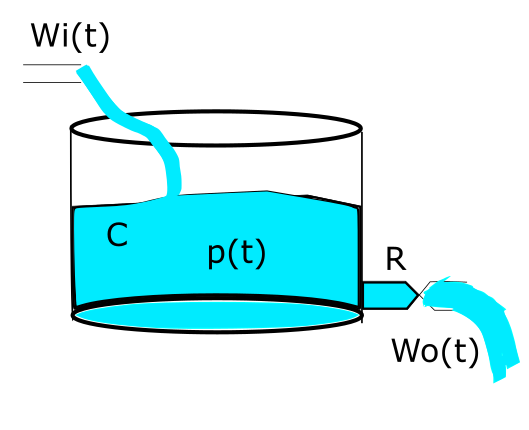
\includegraphics[scale = 0.5]{images/F1}\\
	{fig1-2 Sistema de eléctrico equivalente}
\end{center}


Del sistema mostrado en la fig1-1 se obtuvo el siguiente modelo matemático.
$$Wi(t) = h(t)\frac{rg}{R} + A\frac{dh(t)}{dt}$$
Donde h(t) es la altura que cambia con respecto al tiempo.
\\  
La siguiente figura se muestra el modelo equivalente en un sistema eléctrico (fuerza - corriente) del cual se obtienen ecuaciones similares.

\begin{center}
	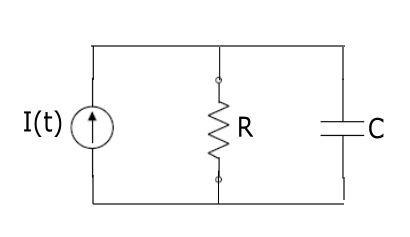
\includegraphics[scale = 0.5]{images/RCI}\\
	{fig1-2 Sistema de eléctrico equivalente}
\end{center}

Las ecuaciones obtenidas del circuito son:

$$i(t) = \frac{v(t)}{R} + C\frac{v(t)}{dt} $$

Aplicamos Laplace a la ecuación anterior.

$$\mathcal{L}[i(t) = \frac{v(t)}{R} + C\frac{v(t)}{dt}]$$
$$I(S) = \frac{V(S)}{R} + sCV(s) $$

Despues de aplicar Laplace encontramos la F.T. (Función de transferencia).\\
La función de transferencia es la salida que en este caso es $\frac{V(S)}{R}$ entre la entrada que es $I(S)$ por lo tanto la función de trasferencia quedaria de la siguiente forma.

$$I(s) = V(s)[\frac{1}{R}+ sC]$$

$$\frac{V(s)}{I(s)} = \frac{1}{\frac{1}{R} + sC}$$

$$\frac{V(S)}{I(S)} = \frac{R}{RCS + 1}$$

$$\frac{Wo(S)}{Wi(S)} = \frac{1}{RCS + 1}$$

donde $Wo(S) = \frac{V(S)}{R}$ y $WI(S) = I(S)$ normalmente los terminos $RC$ se definen como una constante de tiempo llamada tau $(\tau)$. Por la ecuación obtenida podemos decir que es un sistema de primer orden.
\subsection{Programa en scilab para observar el comportamiento de un sistema de primer orden}

Para poder observar el comportamiento de cualquier sistema de primer orden cuando se le aplica un escalon unitario, ya se habia mencionado que siempre tiene la forma : 

$$Y(s) = \frac{bs + c}{s(s + a)}$$

La ecuación anterior la podemos resolver por el método de fracciones parciales.

$$Y(s) = \frac{bs + c}{s(s + a)} = \frac{A}{s} + \frac{B}{s + a}$$

donde al resolver las fracciones parciales se obtuvo que:

$$A = \frac{c}{a} ; B = b - \frac{c}{a}$$

Aplicando la inversa de Laplace

$$\mathcal{L}^{-1}[Y(s) = \frac{A}{s} + \frac{B}{s + a}]$$

$$us(t) = \frac{c}{a} + (b - \frac{c}{a})e^{-at}  $$

Conociendo la ecuación anterior podemos diseñar un programa que nos permita observar el comportamiento de cualquier sistema de primer orden. 
\begin{center}
\begin{verbatim}
function [y] = fun2(a,b,c)
 t = 0:0.1:10;
  y = c/a + (b - c/a)*(exp(-a*t));
   plot(t,y);
endfunction
\end{verbatim}
fig1-3 Código implementado en scilab \cite{Mora}
\end{center} 

Con este programa solo basta con escribir la ecuación de la forma $Y(s) = \frac{bs + c}{s(s + a)}$ para encontrar los valores de a, b y c. \\ \\
Para probar el programa se uso un circuito RC que da un sistema de primer orden donde $\tau$ = 1. 

\begin{verbatim}

--> exec('mifun2.sci',-1)

--> fun2(1,0,1)

\end{verbatim}


\begin{center}
	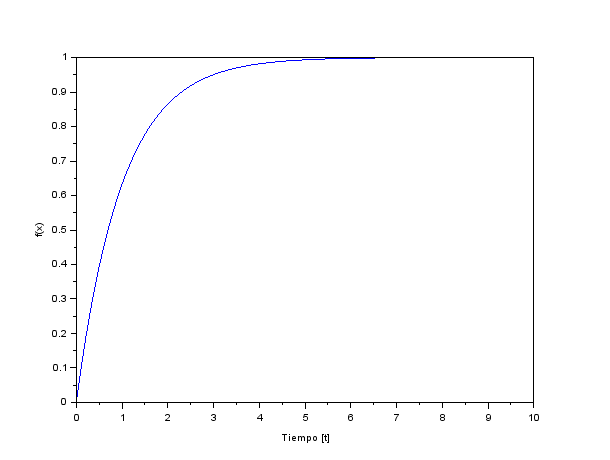
\includegraphics[scale = 0.4]{images/GRAF}\\
	{fig1-4 Respuesta de un circuito RC}
\end{center}

\begin{center}
	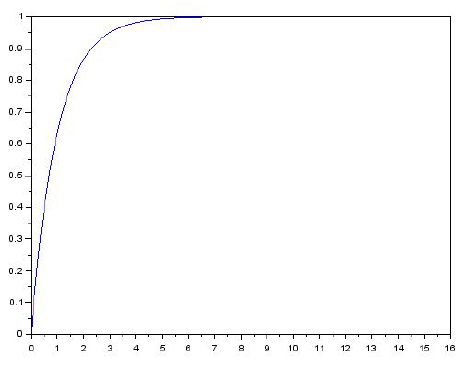
\includegraphics[scale = 0.6]{images/funcionscilab}\\
	{fig1-5 con la funcion scilab}
\end{center}

Con $W_{in}<W_{o}$ obtuvimos lo siguiente:

\begin{center}
	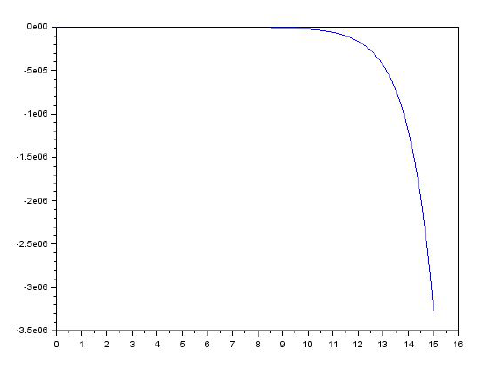
\includegraphics[scale = 0.6]{images/funcionscilab2}\\
	{fig1-6 con la funcion scilab}
\end{center}


\begin{center}
	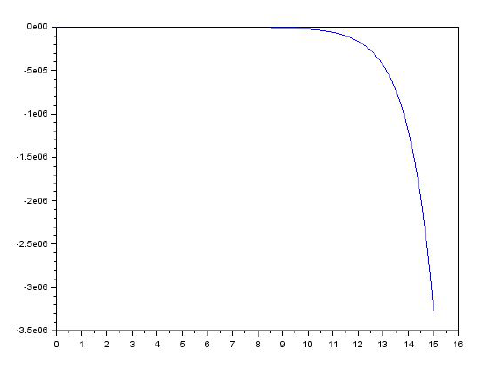
\includegraphics[scale = 0.6]{images/funcionscilab2}\\
	{fig1-7 con nuestro codigo}
\end{center}

Con $W_{in}=W_{o}$ obtuvimos lo siguiente: 

\begin{center}
	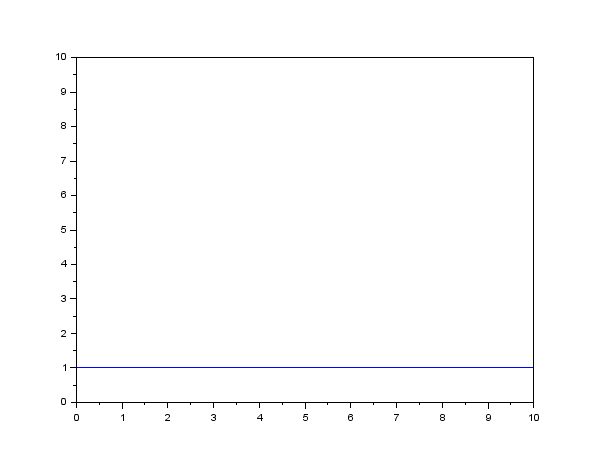
\includegraphics[scale = 0.4]{images/h}\\
	{fig1-8 con nuestro programa cuando entrada y salida de flujo sean iguales}
\end{center}

\section{Conclusiones}
 Erick David Bedolla García\\ \ \\
En esta práctica tuvimos la oportunidad de ver como el control es muy importante hoy en día, ya que la parte de automatización se usa en practicamente todos los sistemas industriales actuales. Se pudo observar que cualquier sistema puede ser determinado por un modelo matemático y simulado con un circuito eléctrico lo cual hace muy práctico ya que podemos ir probando por medio de un circuito en vez de probarlo con un sistema completo que podría fallar y generar muchas perdidas económicas.\\\\\

Hernandez Arteaga Aracely Lizeth\\

con respecto a si es mas grande o mas pequeña la salida dependera por asi decirlo de rR si r es muy grande esta no opondra resistencia al paso del liquido y si es pequeña se opindra probocando que la h se incremente 
La transformada de laplace es importante para lograr visualizar la eciuacion en el dominio de la frecuencia que nos permite determinar la funcion de transferencia para nuestro sistema















 
 




 










\begin{thebibliography}{99}
	\bibitem{Ogata} Ingenieria de Control Moderna , Katsuhiko Ogata, 5a Edición.
	\bibitem{Echeverria} Apuntes Scilab, Rosa Echeverría Líbano, Universidad de Sevilla.
	\bibitem{Mora} Introducción a Scilab, Héctor Manuel Mora Escobar, Universidad Nacional de Colombia Bogotá
\end{thebibliography}

\end{document}
